\section{Introduction}
\label{sec:introduction}

LLM agents are increasingly undertaking complex, long-horizon tasks across real-world environments~\citep{yao2023react,shinn2023reflexion,jimenez2024swebench,gu2024toolsandbox,zhou2024webarena}.
As task horizons expand, evaluating only final output results becomes insufficient to identify agent deficiencies and diagnose failure modes, therefore bringing trajectory-level evaluation to the forefront of agent research~\citep{qian2024agentprocessbench,shi2025earlyeval}.

However, existing trajectory evaluation paradigms face a central granularity problem, especially for long-horizon tasks.
Whole-trajectory verification is too coarse to focus on concrete failures and their associated evidence in long trajectories, whereas atomic-step scoring is too fine-grained: isolated messages lack task context, so ordinary retries and harmless observations become noise.
This granularity gap further raises two challenges.
Agent executions often admit multiple valid and effective paths. Because of this granularity gap, evaluation typically offers only limited path references and therefore struggles to faithfully reflect the quality of diverse agent executions.
Moreover, full-trajectory review delays diagnosis that could be made earlier, so an execution that has already gone wrong may continue, wasting model resources and triggering additional skill or tool calls.

\begin{figure*}[t]
\centering
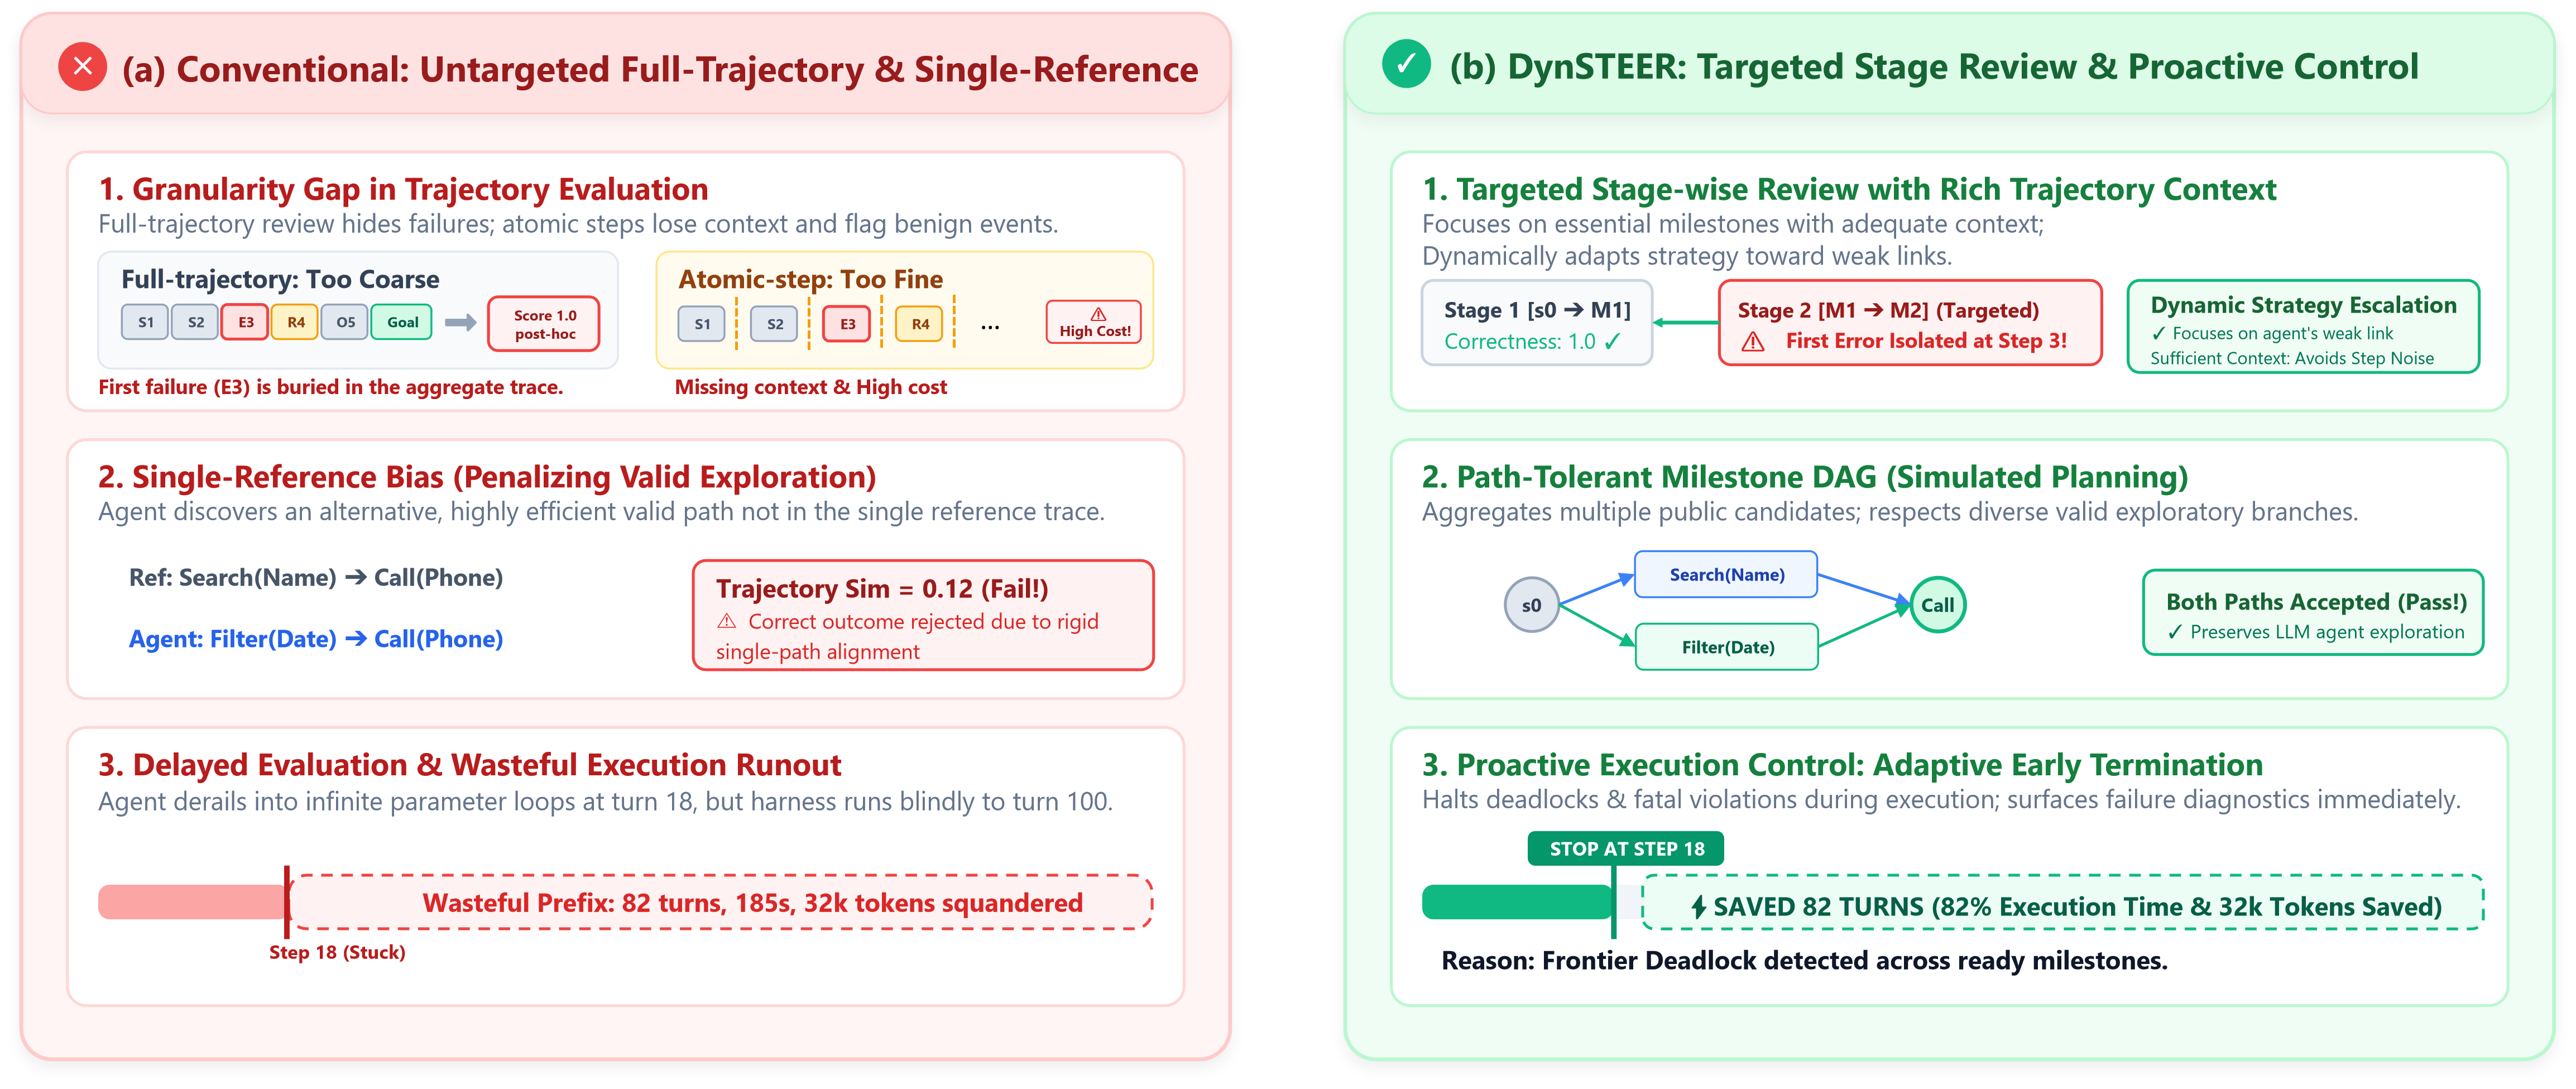
\includegraphics[width=0.96\textwidth]{figures/teaser_comparison.png}
\vspace{-0.25cm}
\caption{\textbf{Comparison of Agent Evaluation Paradigms.} (a) Conventional paradigms evaluate either coarse outcomes or noisy atomic steps, often against a single reference, and discover waste only after execution. (b) \textsc{DynSTEER} evaluates path-tolerant milestone-bounded stages and uses the resulting stage evidence to target review and stop hopeless prefixes early.}
\label{fig:teaser_comparison}
% \vspace{-0.35cm}
\end{figure*}

As illustrated in Figure~\ref{fig:teaser_comparison}, we introduce \textbf{DynSTEER}, a \textsc{Dyn}amic \textbf{S}tage-wise \textbf{T}rajectory \textbf{E}valuation and \textbf{E}xecution-time \textbf{R}eview framework.
To address the granularity challenge, DynSTEER performs stage-wise dynamic evaluation: it segments rollouts at necessary execution nodes, preserves task context while isolating localized evidence for error attribution, and adapts its multi-level review strategy based on stage-level results.
To avoid single-reference bias, it compiles a path-tolerant milestone graph from available task inputs via multi-candidate simulated planning and majority consensus, capturing necessary task invariants while accommodating diverse legitimate paths.
Finally, it supports detecting unrecoverable prefixes and terminating them to curb resource waste.

Experiments on ToolSandbox and SWE-bench Pro show that DynSTEER improves discriminability by 85.2\% and 164.0\% over whole-trajectory evaluation, enhances diagnostic precision, preserves the validity of diverse execution paths, and saves 17.74\% and 8.40\% of execution steps across paired trajectories.

In summary, our contributions are as follows:
\begin{itemize}[leftmargin=*,itemsep=1.5pt,topsep=1pt]
    \item \textbf{Stage-wise Dynamic Evaluation:} We segment rollouts at necessary execution-step nodes and adapt multi-level review routing from stage-level results, isolating context-rich evidence windows for multidimensional scoring and first-error localization.
    \item \textbf{Path-Tolerant Task Blueprint Compilation:} We compile a milestone DAG from available task inputs via multi-candidate planning and strict-majority consensus, preserving diverse valid paths without reference leakage.
    \item \textbf{Counterfactual Early Termination:} We detect unrecoverable prefixes from stage-level evidence and terminate them, substantially reducing wasted computation.
\end{itemize}
